\documentclass[10pt,aspectratio=169]{beamer}

\usetheme[progressbar=frametitle]{metropolis}
\usepackage{appendixnumberbeamer}

\usepackage{booktabs}
\usepackage[scale=2]{ccicons}
\usepackage{pgfplots}
\usepgfplotslibrary{dateplot}

\usepackage{xspace}
\newcommand{\themename}{\textbf{\textsc{metropolis}}\xspace}
\usepackage{color}
\usepackage{printlen}
\usepackage{makecell}
\usepackage{bm}
\usepackage{hyperref}
\usepackage{minted}
\usepackage{multicol}
\usepackage{graphicx}
\usepackage{amssymb}
\definecolor{orange-git}{RGB}{243, 76, 38}
\setbeamertemplate{frame footer}{\color{black!30}{QI Group Meeting - 10/02/2023}}
\makeatletter
\define@key{beamerframe}{gitstandout}[true]{%
\setbeamertemplate{footline}{}%
}
\makeatother
\title{\vspace*{60pt}\LARGE Introduction Tutorial to Git}
\subtitle{QI Group Meeting}
% \date{\today}
\date{10/02/2023}
\author{\large\textbf{Yoann Piétri}}
\institute{LIP6 - Sorbonne Université - CNRS}
\titlegraphic{
\includegraphics[height=0.8cm]{logos/logo-lip6.png}\;
\includegraphics[height=0.8cm]{logos/cnrs-logo.png}\hfill}

\begin{document}
\setbeamercolor{background canvas}{bg=white}

\maketitle

{
    \setbeamercolor{palette primary}{fg=white, bg=orange-git}
    \begin{frame}[standout,gitstandout]
        What is Git?
    \end{frame}
}

\begin{frame}{Git}
    Git is a free and open source \textbf{distributed version control system}.

    \vspace*{\baselineskip}

    \begin{quote}
        It is also impossible to change any file, date, commit message, or any other data in a Git repository without changing the IDs of everything after it.
    \end{quote}
    \begin{flushright}
        \textit{The Pro Git book}
    \end{flushright}

    \begin{multicols}{2}
        \begin{itemize}
            \item Snapshots, Not Differences
            \item Nearly Every Operation Is Local \textit{(Sorry non-locality)}
            \item Git Has Integrity \textit{(Not like us)}
            \item Git Generally Only Adds Data
            \item The Three States (Working directory, Staging area, Repository)
            \item Git is cool
        \end{itemize}
    \end{multicols}
\end{frame}


{
\setbeamercolor{palette primary}{fg=white, bg=orange-git}
\begin{frame}[standout,gitstandout]
    What is not Git?
\end{frame}
}

\begin{frame}{Not Git}
    Git is not:

    \begin{itemize}
        \item A magic solution to everything;
        \item A backup system\footnote{In some specific cases, it may be used at such};
        \item A synchronisation system;
        \item Github, Gitlab or any other tool built on top of Git;
    \end{itemize}
\end{frame}

\begin{frame}{Other version control tools}
    Git is not alone in the world of version controls and here are examples of some other tools:
    \begin{itemize}
        \item Subversion (svn)
        \item CVS
        \item BitKeeper
        \item Fossil
        \item RCS
        \item ...
    \end{itemize}

    Git remains the most use version control system today.
\end{frame}

\begin{frame}[fragile]{Good reads}
    Good reads on Git:

    \begin{itemize}
        \item The Pro Git book \url{https://git-scm.com/book/en/v2} (many things of the presentation are inspired from there)
        \item The git reference manual \url{https://git-scm.com/docs}

    \end{itemize}
\end{frame}

\section{Git basics}

\begin{frame}[fragile]{Start of a project example}
    \begin{minted}[mathescape,gobble=2, linenos, frame=lines]{bash}
    $ git init -b main
    $ git config --local user.email "Yoann.Pietri@lip6.fr"
    $ touch README.md
    $ git add README.md
    $ git commit -m "Initial commit"
      \end{minted}
    \begin{multicols}{2}
        \begin{enumerate}
            \item Initialize the repository with branch \verb|main|
            \item Configure the local (for current git repository) email
            \item Create a file name \verb|README.md|
            \item Add the file to the staging area (see later), i.e. what's going to be committed
            \item Commit
        \end{enumerate}
    \end{multicols}
\end{frame}

{
\setbeamercolor{palette primary}{fg=white, bg=orange-git}
\begin{frame}[standout,gitstandout]
    What is a commit?
\end{frame}
}

\begin{frame}[fragile]{Commit}
    A commit is a \textbf{snapshot} (i.e. a picture) of your code at a given moment.

    Unlike other version control systems, Git does not only store the difference between versions, each commit represents the full code, and git think you repository as a series of commits.

    It makes git a miniature file system, with version control, integrity and powerful tools.

    \textit{Snapshots, Not Differences}
\end{frame}

\begin{frame}[fragile]{Integrity}
    Let's show the commit history of our simple earlier project:
    \begin{minted}[mathescape,gobble=2, linenos, frame=lines]{bash}
    $ git log
    commit 13d588fd13f50a8554dfc6cb06d83b689c82ef81 (HEAD -> main)
    Author: Yoann Piétri <Yoann.Pietri@lip6.fr>
    Date:   Wed Dec 28 11:08:29 2022 +0100

    Initial commit
    \end{minted}

    What is \verb|13d588fd13f50a8554dfc6cb06d83b689c82ef81| ?
\end{frame}

\begin{frame}[fragile]{Integrity}
    At commit, Git takes into his snapshot everything in the staging area, along with some metadata (commit name, committer information, date etc) and secure it in a secure manner and \textbf{generates a unique checksum}.

    Any change on the commit will make this checksum change.
\end{frame}


\begin{frame}[fragile]{Integrity}
    Let's show the commit history of our simple earlier project:
    \begin{minted}[mathescape,gobble=2, linenos, frame=lines]{bash}
    $ git commit --amend -m "Almost intial commit"
    $ git log
    commit 95129c0bd7ed42a458773d9fa4d6406d268a6161 (HEAD -> main)
    Author: Yoann Piétri <Yoann.Pietri@lip6.fr>
    Date:   Wed Dec 28 11:08:29 2022 +0100

    Almost intial commit
    \end{minted}

    \verb|95129c0bd7ed42a458773d9fa4d6406d268a6161| $\neq$ \verb|13d588fd13f50a8554dfc6cb06d83b689c82ef81|
\end{frame}

\begin{frame}[fragile]{Integrity}
    \begin{quote}
        It is also impossible to change any file, date, commit message, or any other data in a Git repository without changing the IDs\footnote{The checksums are also the IDs of the git objects} of everything after it.
    \end{quote}
    \begin{flushright}
        \textit{The Pro Git book}
    \end{flushright}

    \textit{Git Has Integrity}
\end{frame}

\begin{frame}[fragile]{Not screwing things up}
    \begin{quote}
        When you do actions in Git, nearly all of them only add data to the Git database. It is hard\footnote{Hard doesn't mean impossible} to get the system to do anything that is not undoable or to make it erase data in any way.

        This makes using Git a joy because we know we can experiment without the danger of severely screwing things up\footnote{Still possible though}.
    \end{quote}
    \begin{flushright}
        \textit{The Pro Git book}
    \end{flushright}

    \textit{Git Generally Only Adds Data}
\end{frame}

\section{The (almost) 3 states}

\begin{frame}[fragile]{The 3 states}
    Git has 3 states and 3 associated regions
    \begin{multicols}{2}
        \begin{itemize}
            \item Modified
            \item Staged
            \item Committed
            \item Working Directory
            \item Staging area
            \item Repository
        \end{itemize}
    \end{multicols}
\end{frame}

\begin{frame}[fragile]{The 3 states}
    \begin{figure}
        \includegraphics[scale=0.13]{Schemas/Schémas Git-01.jpg}
    \end{figure}
\end{frame}

\begin{frame}[fragile]{The hidden state}
    What if, in the middle of implementing a feature, you need to work on another branch, or implement an hotfix ? Stashing is here for you.

    \vspace*{\baselineskip}

    \begin{quote}
        Stashing takes the dirty state of your working directory and saves it on a stack of unfinished changes that you can reapply at any time (even on a different branch).
    \end{quote}
    \begin{flushright}
        \textit{The Pro Git book}
    \end{flushright}
\end{frame}

\begin{frame}[fragile]{The hidden state}
    \begin{figure}
        
\includegraphics[scale=0.45]{memes/meme-4-states.jpg}
    \end{figure}
\end{frame}


\begin{frame}[fragile]{The hidden state}
    \begin{minted}[mathescape,gobble=2, linenos, frame=lines]{bash}
    $ git status
        On branch main
        nothing to commit, working tree clean
    $ touch unfinished_work
    $ git status
        On branch main
        Untracked files:
            unfinished_work

    $ ls
        README.md  unfinished_work
    \end{minted}
\end{frame}

\begin{frame}[fragile]{The hidden state}
    \begin{minted}[mathescape,gobble=2, linenos, frame=lines]{bash}
    $ git add unfinished_work
    $ git stash
        Saved working directory and index state WIP on main: b0f26d4 Initial commit
    $ git status
        On branch main
        nothing to commit, working tree clean
    $ ls
       README.md
    $ git stash list
    stash@{0}: WIP on main: b0f26d4 Initial commit
    \end{minted}
\end{frame}

\begin{frame}[fragile]{The hidden state}
    \begin{minted}[mathescape,gobble=2, linenos, frame=lines]{bash}
    $ git stash apply
        On branch main
        Changes to be committed:
            new file:   unfinished_work
    $ ls
        README.md  unfinished_work
    \end{minted}

    \begin{minted}[mathescape,gobble=2, linenos, frame=lines]{bash}
    $ git stash drop
        Dropped refs/stash@{0} (3fd9e24718f373740c72398833fb1be353586246)
    \end{minted}
\end{frame}

\begin{frame}[fragile]{The hidden state}
    \begin{figure}
        \includegraphics[scale=0.13]{Schemas/Schémas Git-02.jpg}
    \end{figure}
\end{frame}


\begin{frame}[fragile]{The Three States}
    \begin{quote}
        Pay attention now - here is the main thing to remember about Git if you want the rest of your learning process to go smoothly. Git has three main states [...]
    \end{quote}
    \begin{flushright}
        \textit{The Pro Git book}
    \end{flushright}

    \textit{The Three States}
\end{frame}

\begin{frame}[fragile]{The forgotten modifications}
    \begin{figure}
        
\includegraphics[scale=0.35]{memes/meme-stashed.jpg}
    \end{figure}
\end{frame}

\section{Branches}

 {
  \setbeamercolor{palette primary}{fg=white, bg=orange-git}
  \begin{frame}[standout,gitstandout]
      What is a commit?\\ (déjà-vu ?)
  \end{frame}
 }

\begin{frame}[fragile]{Commit}
    A commit is a \textbf{snapshot} of your staged work along with some metadata for the commit (author, data, message) and \textbf{one ore more parent commit(s)}.

    \begin{figure}
        \centering
        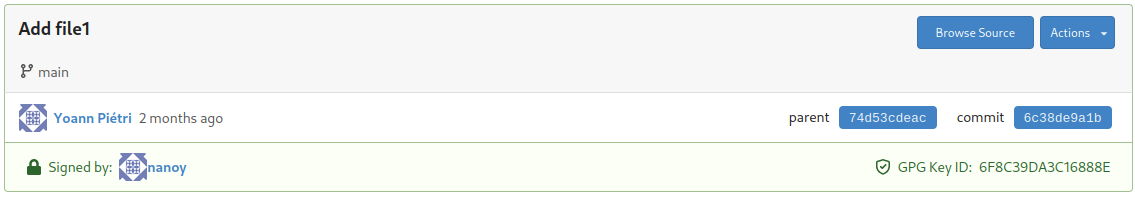
\includegraphics[scale=0.35]{parent_commit.png}
    \end{figure}
\end{frame}

\begin{frame}[fragile]{Branches}
    \begin{figure}
        \includegraphics[scale=0.15]{Schemas/Schémas Git-03.jpg}
    \end{figure}
\end{frame}

\begin{frame}[fragile]{Branch}
    \begin{minted}[mathescape,gobble=2, linenos, frame=lines]{bash}
    $ git checkout -b main2
        Switched to a new branch 'main2'
    $ touch file2
    $ git add file2
    $ git commit -m "Add file2"
    $ git checkout main
        Switched to branch 'main'
    $ touch file1
    $ git add file1
    $ git commit -m "Add file1"
    \end{minted}
\end{frame}

\begin{frame}[fragile]{Branch}
    \begin{minted}[mathescape,gobble=2, linenos, frame=lines]{bash}
    $ git log --graph --oneline --all
        * 6c38de9 (HEAD -> main) Add file1
        | * ed86875 (main2) Add file2
        |/
        * 95129c0 Almost intial commit
    \end{minted}
\end{frame}


{
\setbeamercolor{palette primary}{fg=white, bg=orange-git}
\begin{frame}[standout,gitstandout]
    What is a branch?
\end{frame}
}

\begin{frame}[fragile]{Branch}
    A branch is a \textbf{lightwight movable pointer} to one of the project's commits.

    When you commit on a branch, the pointer moves to the new commit.

    When you create a commit from a branch A, you create an additional pointer B that points to the same commit as A, at the beginning.
\end{frame}


{
\setbeamercolor{palette primary}{fg=white, bg=orange-git}
\begin{frame}[standout,gitstandout]
    What is HEAD?
\end{frame}
}

\begin{frame}[fragile]{HEAD}
    Head is special pointer pointing to the current branch (could also point to a specific commit in certain case). It's also where the next commit will be added.

    \begin{minted}[mathescape,gobble=2, linenos, frame=lines]{bash}
    $ git log --graph --oneline --all
        * 6c38de9 (HEAD -> main) Add file1
        | * ed86875 (main2) Add file2
        |/
        * 95129c0 Almost intial commit
    \end{minted}

    \begin{minted}[mathescape,gobble=2, linenos, frame=lines]{bash}
    $ git checkout main2
    $ git log --graph --oneline --all
        * 6c38de9 (main) Add file1
        | * ed86875 (HEAD -> main2) Add file2
        |/
        * 95129c0 Almost intial commit
    \end{minted}

\end{frame}

\begin{frame}[fragile]{HEAD}
    \begin{figure}
        \includegraphics[scale=0.15]{Schemas/Schémas Git-05.jpg}
    \end{figure}
\end{frame}

\section{Bringing back those branches together}

\begin{frame}[fragile]{Why branches?}
    \begin{quote}
        Branching means you diverge from the main line of development and continue to do work without messing with that main line.
    \end{quote}
    \begin{flushright}
        \textit{The Pro Git book}
    \end{flushright}

    At some point, you might want to integrate your change in the main line of development.
\end{frame}

\begin{frame}[fragile]{Merge}
    Merging
    \begin{itemize}
        \item is asymmetrical (one target, and one source)
        \item creates a merging commit (having the target and source commit has parents)
        \item is not destructive (the source branch still exists after ward)
    \end{itemize}
\end{frame}

\begin{frame}[fragile]{Merge}
    \begin{minted}[mathescape,gobble=2, linenos, frame=lines]{bash}
    $ git log --graph --oneline --all
        * 6c38de9 (HEAD -> main) Add file1
        | * ed86875 (main2) Add file2
        |/
        * 95129c0 Almost intial commit
    \end{minted}

    \begin{minted}[mathescape,gobble=2, linenos, frame=lines]{bash}
    $ git merge main2 -m "Merge commit"
    $ git log --graph --oneline --all
        *   39bd944 (HEAD -> main) Merge commit
        |\
        | * ed86875 (main2) Add file2
        * | 6c38de9 Add file1
        |/
        * 95129c0 Almost intial commit
    \end{minted}

\end{frame}

\begin{frame}[fragile]{HEAD}
    \begin{figure}
        \includegraphics[scale=0.15]{Schemas/Schémas Git-06.jpg}
    \end{figure}
\end{frame}

\begin{frame}[fragile]{Merge conflicts}
    \begin{figure}
        \centering
        
\includegraphics[scale=0.8]{memes/meme-conflicts.jpg}
    \end{figure}
\end{frame}

\begin{frame}[fragile]{Merge conflicts}
    \begin{quote}
        Occasionally, this process doesn't go smoothly. If you changed the same part of the same file differently in the two branches you're merging, Git won't be able to merge them cleanly.
    \end{quote}
    \begin{flushright}
        \textit{The Pro Git book}
    \end{flushright}

    You have to manually select which changes yout want to keep from each branch and then do the merge commit.
\end{frame}

\begin{frame}[fragile]{Rebasing}
    \begin{quote}
        In Git, there are two main ways to integrate changes from one branch into another: the merge and the rebase.
    \end{quote}
    \begin{flushright}
        \textit{The Pro Git book}
    \end{flushright}

    \begin{minipage}{0.49\textwidth}
        \textbf{Merging}
        \begin{itemize}
            \item Non-linear history
            \item Keep all previous commits
            \item Create a merge commit
        \end{itemize}
    \end{minipage}
    \begin{minipage}{0.49\textwidth}
        \textbf{Rebasing}
        \begin{itemize}
            \item Linear history
            \item Create new commits with same modification and delete old commits
            \item Does not create a merge commit
        \end{itemize}
    \end{minipage}
\end{frame}

\begin{frame}[fragile]{Before rebase}
    \begin{minted}[mathescape,gobble=2, linenos, frame=lines]{bash}
    $ git log --graph --oneline --all
        * 3fb7dfb (HEAD -> main) C4
        | * 6008b93 (my_fix) C3
        | * e60ea6c C2
        |/
        * adb048b C1
        * ccee678 C0
    \end{minted}
\end{frame}

\begin{frame}[fragile]{HEAD}
    \begin{figure}
        \includegraphics[scale=0.15]{Schemas/Schémas Git-07.jpg}
    \end{figure}
\end{frame}

\begin{frame}[fragile]{Rebase my\_fix on main}
    \begin{minted}[mathescape,gobble=2, linenos, frame=lines]{bash}
    $ git checkout my_fix
    $ git rebase main
    $ git log --graph --oneline --all
        * 6efb6ee (my_fix) C3
        * 7bece1a C2
        * 3fb7dfb (HEAD -> main) C4
        * adb048b C1
        * ccee678 C0
    \end{minted}

    Linear history, but checksums different.
\end{frame}

\begin{frame}[fragile]{HEAD}
    \begin{figure}
        \includegraphics[scale=0.15]{Schemas/Schémas Git-08.jpg}
    \end{figure}
\end{frame}

\begin{frame}[fragile]{Fast-forward merge}
    \begin{minted}[mathescape,gobble=2, linenos, frame=lines]{bash}
    $ git checkout main
    $ git merge my_fix
        Updating 3fb7dfb..6efb6ee
        Fast-forward
    $ git log --graph --oneline --all
        * 6efb6ee (HEAD -> main, my_fix) C3
        * 7bece1a C2
        * 3fb7dfb C4
        * adb048b C1
        * ccee678 C0
    \end{minted}

    Fast-foward: merge that does create a merge commit (just moves the pointer, in case of a linear history).
\end{frame}

\begin{frame}[fragile]{HEAD}
    \begin{figure}
        \includegraphics[scale=0.15]{Schemas/Schémas Git-09.jpg}
    \end{figure}
\end{frame}

{
\setbeamercolor{palette primary}{fg=white, bg=orange-git}
\begin{frame}[standout,gitstandout]
    What if someone started a branch on a commit that was rebased after ?\\
\end{frame}
}

\begin{frame}[fragile]{The Perils of Rebasing}
    \begin{quote}
        Ahh, but the bliss of rebasing isn't without its drawbacks, which can be summed up in a single line:

        \textbf{Do not rebase commits that exist outside your repository and that people may have based work on.}

        If you follow that guideline, you'll be fine. If you don't, people will hate you, and you'll be scorned by friends and family.
    \end{quote}
    \begin{flushright}
        \textit{The Pro Git book}
    \end{flushright}
\end{frame}

\section{Revert and blame}

\begin{frame}[fragile]{Revert}
    What if someone (including you) made a bad commit ? You can easily correct by reverting a commit.

    Revert will create a commit for you that undo the modification.

    \textbf{You should (almost) never just delete a commit and force push it\footnote{You can delete commits as long as they have not been pushed to remotes.}}
\end{frame}

\begin{frame}[fragile]{Revert}
    \begin{minted}[mathescape,gobble=2, linenos, frame=lines]{bash}
        $ touch C1
        $ git add C1
        $ git commit -m "C1"
        $ ls
            C0  C1
        $ git log --graph --oneline --all
            * 76cb4f7 (HEAD -> main) C1
            * 0f3e78a C0
        $ git revert 76cb4f7
        $ ls
            C0
        $ git log --graph --oneline --all
            * fb72e86 (HEAD -> main) Revert "C1"
            * 76cb4f7 C1
            * 0f3e78a C0
        \end{minted}
\end{frame}

\begin{frame}[fragile]{HEAD}
    \begin{figure}
        \includegraphics[scale=0.15]{Schemas/Schémas Git-10.jpg}
    \end{figure}
\end{frame}

{
\setbeamercolor{palette primary}{fg=white, bg=orange-git}
\begin{frame}[standout,gitstandout]
    Who fucked up this code?
\end{frame}
}

\begin{frame}[fragile]{Blame}
    git blame shows what revision and author last modified each line of a file

    \begin{minted}[mathescape,gobble=2, linenos, frame=lines]{bash}
    $ git blame alice.py -L 61,63
        f7fafba9 (Yoann Piétri 2023-02-05 14:43:50 +0100 61)
        f7fafba9 (Yoann Piétri 2023-02-05 14:43:50 +0100 62)
        f7fafba9 (Yoann Piétri 2023-02-05 14:43:50 +0100 63)
    \end{minted}
\end{frame}

\begin{frame}[fragile]{Blame}
    \begin{figure}
        \centering
        
\includegraphics[scale=0.4]{memes/meme-git-blame.jpg}
    \end{figure}
\end{frame}

\section{Local and non-local operations}

\begin{frame}[fragile]{Remotes}
    \begin{quote}
        Remote repositories are versions of your project that are hosted on the Internet or network somewhere. You can have several of them, each of which generally is either read-only or read/write for you.
    \end{quote}
    \begin{flushright}
        \textit{The Pro Git book}
    \end{flushright}
\end{frame}

\begin{frame}[fragile]{Remotes}
    We assume the name of the remote to be origin.
    \begin{itemize}
        \item \verb|git remote show origin|: inspect the remote origin
        \item \verb|git push|: Push your work to the remote
        \item \verb|git fetch|: Fetch the new work form the remote
        \item \verb|git pull|: Fetch the new work and merge it to the local branch
    \end{itemize}

    If there is no new commit, \verb|git pull| will only do a fast-forward merge and no merge commit will be created.
\end{frame}

\begin{frame}[fragile]{HEAD}
    \begin{figure}
        \includegraphics[scale=0.15]{Schemas/Schémas Git-11.jpg}
    \end{figure}
\end{frame}

\begin{frame}[fragile]{HEAD}
    \begin{figure}
        \includegraphics[scale=0.15]{Schemas/Schémas Git-12.jpg}
    \end{figure}
\end{frame}

{
\setbeamercolor{palette primary}{fg=white, bg=orange-git}
\begin{frame}[standout,gitstandout]
    As a rule of thumb, never force push to a remote repository\\(I see you Paolo)
\end{frame}
}

\begin{frame}[fragile]{Force push}
    \begin{figure}
        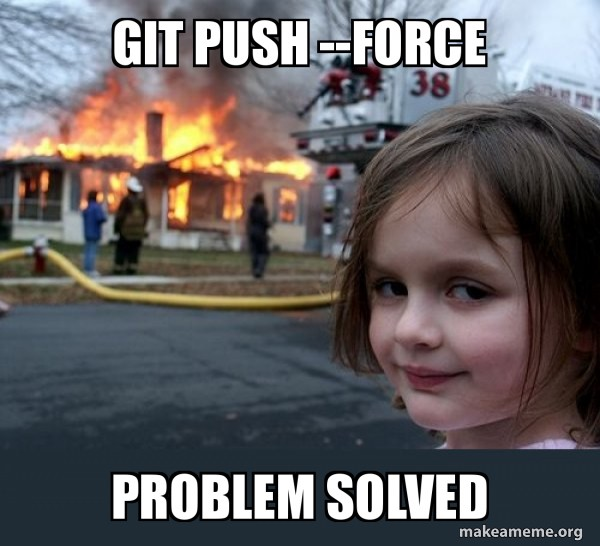
\includegraphics[scale=0.35]{memes/meme-git-force.jpg}
    \end{figure}
\end{frame}

\begin{frame}[fragile]{Git is local}
    \begin{quote}
        Most operations in Git need only local files and resources to operate - generally no information is needed from another computer on your network.

        \vspace*{\baselineskip}

        To browse the history of the project, Git doesn't need to go out to the server to get the history and display it for you - it simply reads it directly from your local database.

        \vspace*{\baselineskip}

        This also means that there is very little you can't do if you're offline or off VPN. If you get on an airplane or a train and want to do a little work, you can commit happily.
    \end{quote}
    \begin{flushright}
        \textit{The Pro Git book}
    \end{flushright}

    \textit{Nearly Every Operation Is Local}
\end{frame}

\section{Conclusion}

\begin{frame}[fragile]{Some cool stuff we didn't talk about}
    \begin{multicols}{2}
        \begin{itemize}
            \item Reset
            \item Tags
            \item Hooks
            \item Git on the Server
            \item Signing
            \item Cherry-picking
            \item Submodules
            \item Internals of Git
            \item Rewriting history (other than rebase)
            \item Stuff I don't even now about
        \end{itemize}
    \end{multicols}
\end{frame}


\begin{frame}[fragile]{Conclusion}
    Git is a free and open source \textbf{distributed version control system}.

    \vspace*{\baselineskip}

    \begin{quote}
        It is also impossible to change any file, date, commit message, or any other data in a Git repository without changing the IDs of everything after it.
    \end{quote}
    \begin{flushright}
        \textit{The Pro Git book}
    \end{flushright}

    \begin{multicols}{2}
        \begin{itemize}
            \item Snapshots, Not Differences \checkmark
            \item Nearly Every Operation Is Local \textit{(Sorry non-locality)} \checkmark
            \item Git Has Integrity \textit{(Not like us)} \checkmark
            \item Git Generally Only Adds Data \checkmark
            \item The Three States (Working directory, Staging area, Repository) \checkmark
            \item Git is cool \checkmark
        \end{itemize}
    \end{multicols}
\end{frame}

\section{The challenge}

\begin{frame}[fragile]{The challenge - Goal}
    The goal is to find a string that looks like this

    \begin{center}
        \verb|${CTF}NIPDt9MI0itWJD3FDBvxUBV7RQ9VNa|
    \end{center}
    (it's start with \verb|${CTF}| and the rest is (almost) random).

    \textbf{You only have to use git commands.} You might also use the \verb|cat| command to print the content of a file.

    If you need authentification at some point, everything will be already set in place so you don't have to enter any password.

    You can now find the useful code here: \url{https://github.com/nanoy42/git-ctf}
\end{frame}

\begin{frame}{License}

    Get the source of this presentation here:

    \begin{center}\url{https://github.com/nanoy42/git-presentation}\end{center}

    Origin of memes is written on the images.

    Quotes where taken from the Git Pro Book.

    The presentation uses the metropolis theme (\url{https://github.com/matze/mtheme}).

    The rest of this presentation is licensed under the
    \href{http://creativecommons.org/licenses/by-sa/4.0/}{Creative Commons
        Attribution-ShareAlike 4.0 International License}.

    \begin{center}\ccbysa\end{center}

\end{frame}

\section{List of useful commands}

\begin{frame}[fragile]{List of useful commands}
    \begin{multicols}{2}
        \begin{itemize}
            \item \verb|git commit|
            \item \verb|git add|
            \item \verb|git init|
            \item \verb|git log|
            \item \verb|git remote|
            \item \verb|git blame|
            \item \verb|git push|
            \item \verb|git pull|
            \item \verb|git fetch|
            \item \verb|git merge|
            \item \verb|git rebase|
            \item \verb|git revert|
            \item \verb|git reset|
            \item \verb|git mv|
            \item \verb|git rm|
            \item \verb|git stash|
        \end{itemize}
    \end{multicols}
\end{frame}

\end{document}